\chapter{AI Component Design}
\label{chap:ai-component-design}

This chapter details the design and integration of Artificial Intelligence (AI) components within the \usevar{\srsTitle} system. Understanding where AI fits into the overall workflow and the specific goals it aims to achieve is crucial for effective development and evaluation. The following sections outline the analysis, design, implementation, and evaluation considerations for the AI modules.

\section{Business Context and AI Integration}
\label{section:ai-integration-context}

\usevar{\srsTitle} tackles the complex challenge of tracking individuals across multiple camera views in environments like campuses and factories. The core task requires recognizing and associating individuals as they move between potentially non-overlapping camera fields, often amidst changing appearances, viewpoints, lighting conditions, and occlusions. This inherent complexity and real-world variability make manual tracking labor-intensive, error-prone, and difficult to address effectively with traditional rule-based programming. Artificial Intelligence is therefore central to \usevar{\srsTitle}, providing the automation necessary to significantly improve this process.

The primary AI-driven workflow resides within the system's backend processing core, orchestrated by a service like FastAPI. This workflow involves several key AI steps:
\begin{enumerate}
    \item \textbf{Person Detection:} Identifying individuals within each camera frame using models like Faster R-CNN.
    \item \textbf{Intra-Camera Tracking:} Maintaining consistent temporary IDs for detected individuals within a single camera's view over consecutive frames, utilizing algorithms such as ByteTrack.
    \item \textbf{Feature Extraction for Re-ID:} Generating unique appearance embeddings (features) from detected person images when necessary (e.g., for new tracks or potential handoffs) using models like OSNet.
    \item \textbf{Cross-Camera Re-Identification (Re-ID):} Matching these appearance embeddings across different camera views and time gaps to assign a persistent global identity, linking temporary tracks together.
    \item \textbf{Spatial Mapping:} Transforming the detected location of individuals from the camera's 2D image plane onto a unified top-down map coordinate system, often using techniques like Homography.
\end{enumerate}
These AI components perform the essential visual analysis and identity association. Figure \ref{fig:ai-architecture-overview} provides a high-level illustration of this system architecture and the integration points for these AI modules.

\begin{figure}[!htb] % Use !htb to suggest placement: here, top, bottom
    \centering
    % Use \makebox or adjust width as needed for centering wide figures
    \makebox[\textwidth][c]{
        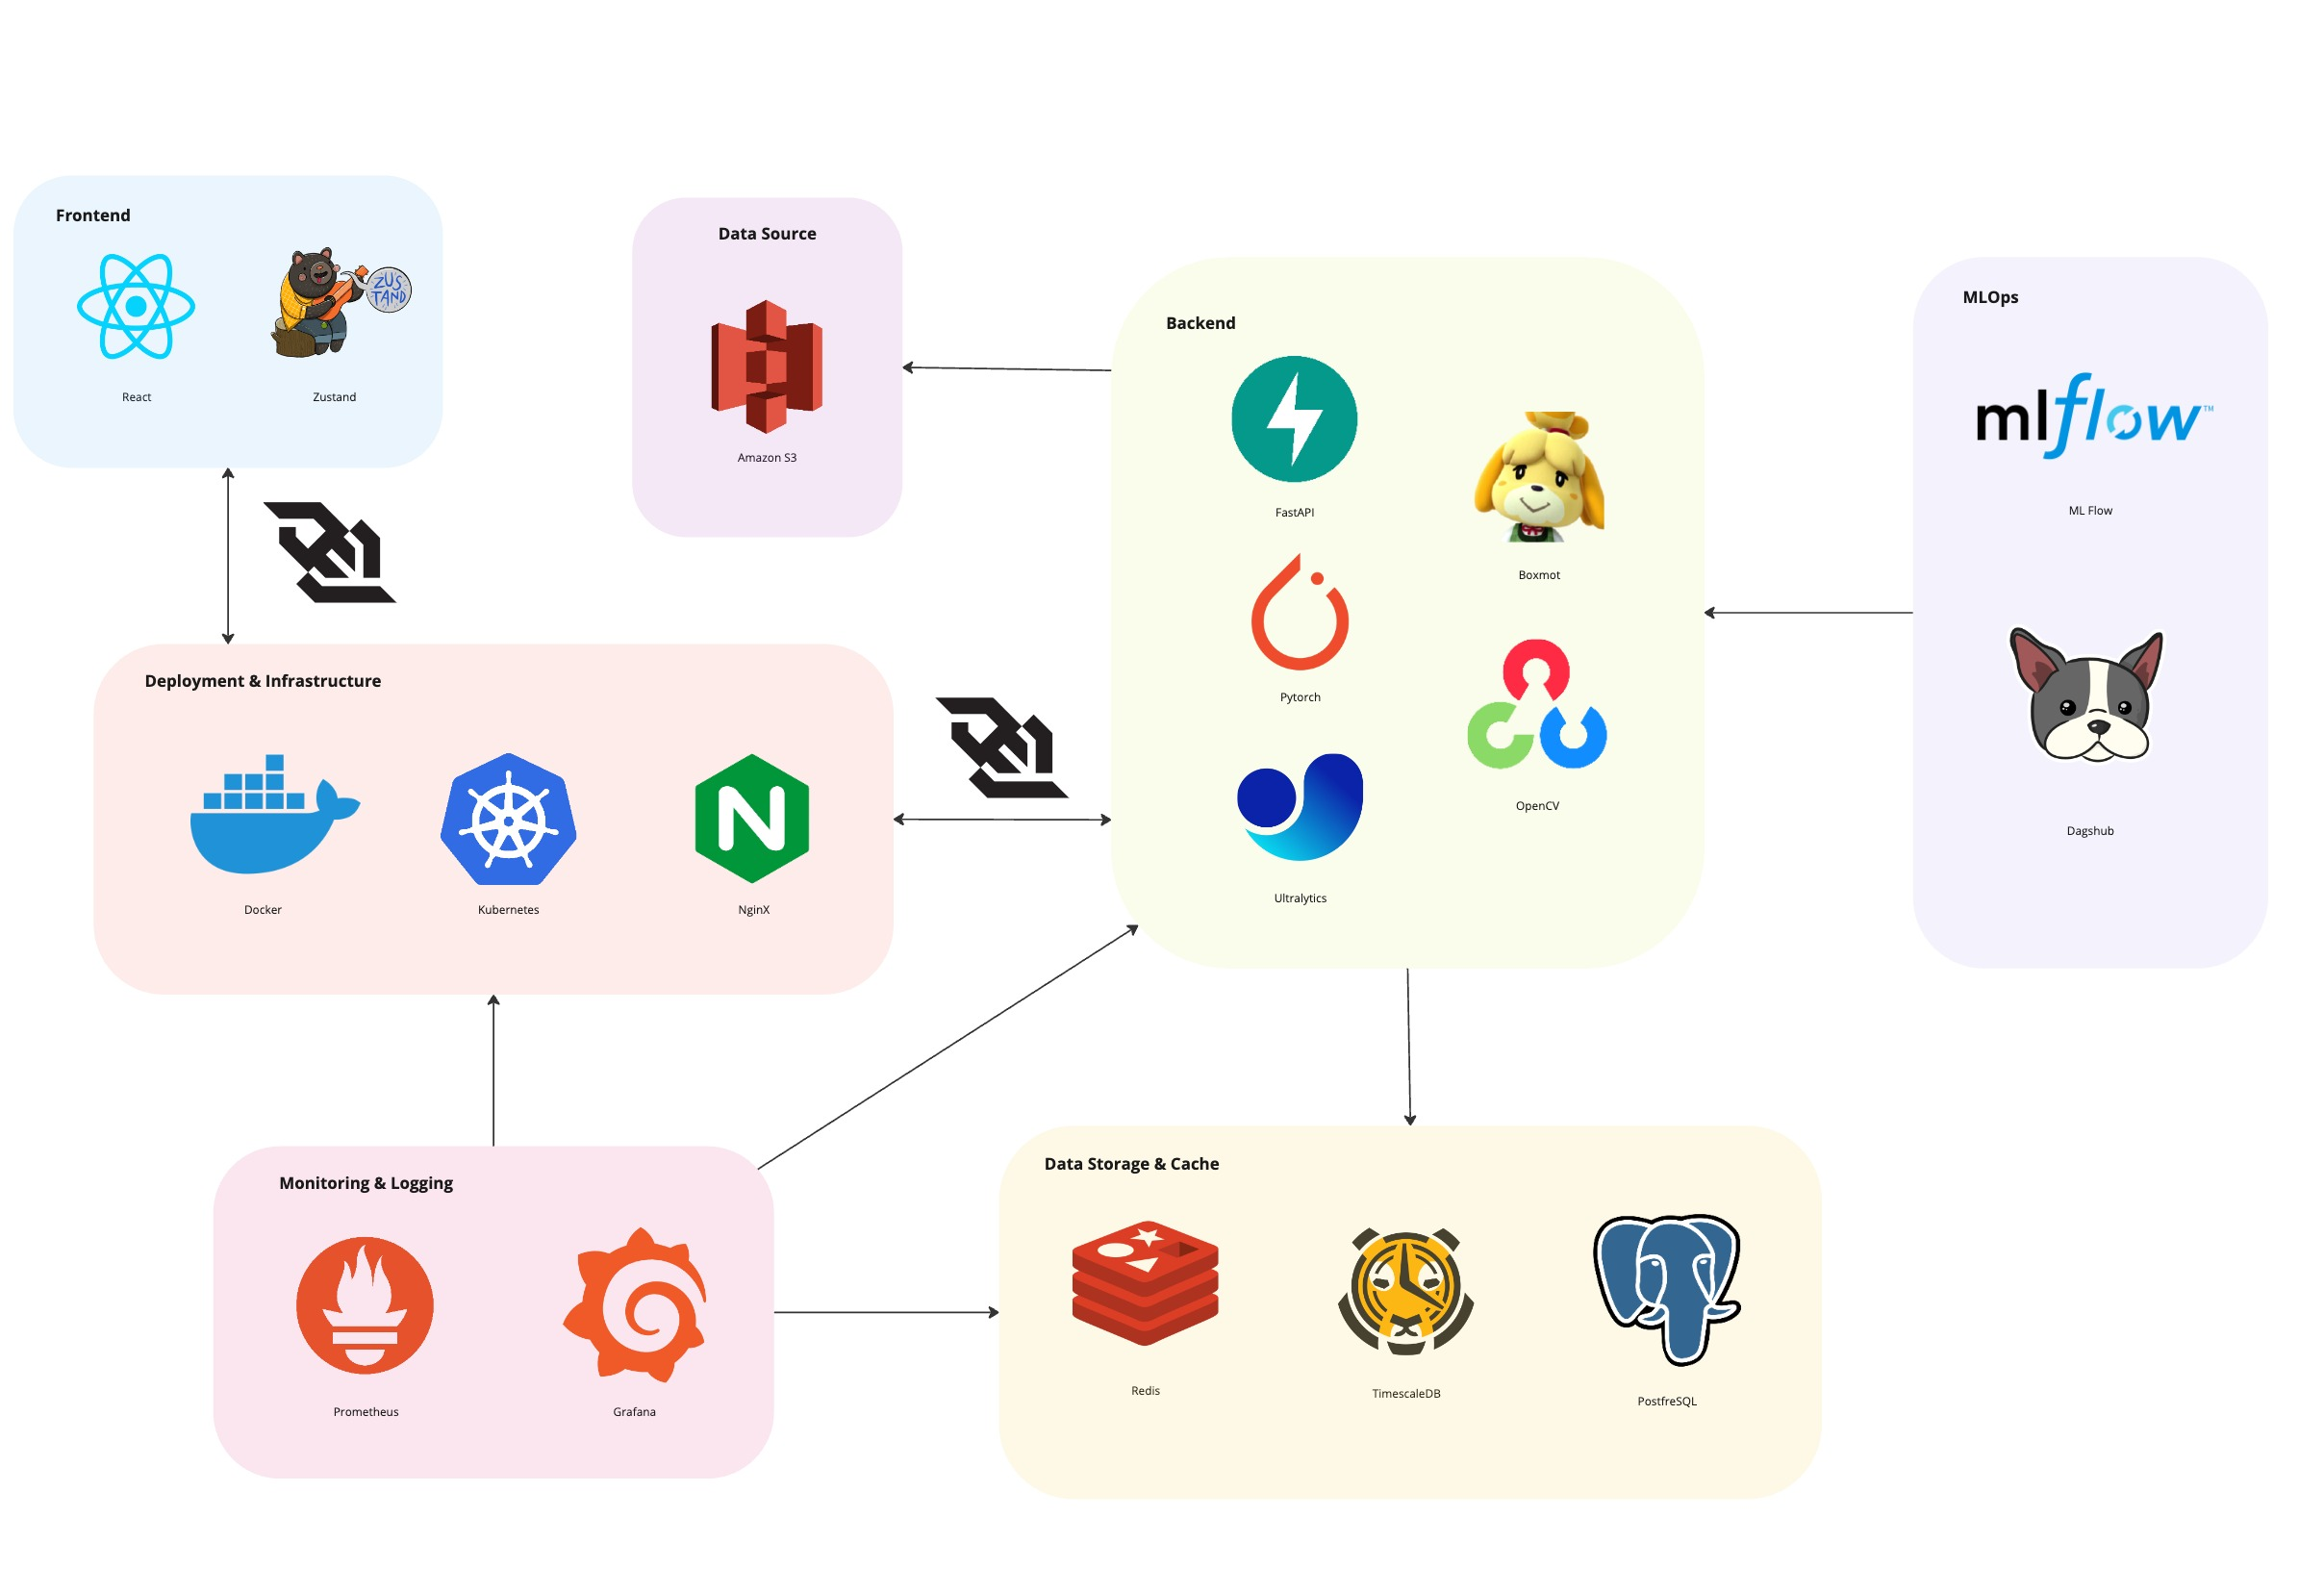
\includegraphics[width=1.0\textwidth, keepaspectratio]{jubjones/architecture.jpg}
    }
    \caption{System Architecture Overview Highlighting AI Component Integration}
    \label{fig:ai-architecture-overview}
\end{figure}
\clearpage % Ensure figure placement doesn't clash excessively with text

The justification for employing AI stems from the nature of the problem itself:
\begin{itemize}
    \item \textbf{Complexity Beyond Rules:} Recognizing and matching people under diverse visual conditions involves intricate pattern recognition that surpasses the capabilities of predefined rules. AI models excel at learning these complex patterns directly from data.
    \item \textbf{Scalability Requirement:} Manually monitoring and correlating feeds from numerous cameras is impractical. AI offers an automated solution capable of handling large data volumes and multiple camera streams simultaneously.
    \item \textbf{Adaptability to Dynamic Environments:} Real-world surveillance scenarios are constantly changing. AI, particularly deep learning, offers better generalization and adaptation to variations in lighting, crowds, and individual appearances compared to static algorithms.
    \item \textbf{Value Despite Imperfection:} Achieving flawless accuracy in cross-camera tracking is exceptionally difficult due to the inherent ambiguities and challenges (e.g., severe occlusions, drastic appearance changes). However, an AI system achieving high, albeit imperfect, accuracy still delivers significant value. It drastically reduces the manual workload for operators and provides a level of situational awareness unattainable through manual means or simpler systems. Even with occasional errors, such as false positive matches or missed detections, the system's ability to automatically correlate identities across most views aligns with the primary goal of enhancing operational efficiency and speeding up investigations. The objective is a substantial improvement over the baseline, accepting a trade-off where occasional inaccuracies are outweighed by the overall gains in automation and insight.
\end{itemize}



\section{Goal Hierarchy}
\label{section:goal-hierarchy}

Ensuring the AI components effectively contribute to the overall success of \usevar{\srsTitle} requires aligning goals across multiple levels, from the high-level organizational objectives down to the specific performance targets of the AI models themselves. This hierarchical approach clarifies the purpose of each component and provides measurable targets for development and evaluation.

The goals are structured as follows:
\begin{itemize}
    \item \textbf{Organization Goals:} Focus on broad impacts like enhancing safety, improving operational efficiency, optimizing resource use, and reducing costs associated with manual monitoring.
    \item \textbf{System Goals (\usevar{\srsTitle}):} Define the overall capabilities of the software, such as accurate cross-camera tracking, persistent identity maintenance, clear path visualization, efficient retrospective analysis, and system usability/reliability.
    \item \textbf{User Goals:} Reflect the specific needs of different user roles:
        \begin{itemize}
            \item \textit{Security Officer:} Faster POI location/monitoring, efficient evidence gathering, reduced manual correlation effort. (\ref{userstory:1}, \ref{userstory:2}, \ref{userstory:5})
            \item \textit{Facility Manager:} Understanding pedestrian flow, identifying bottlenecks, optimizing space. (\ref{userstory:3})
            \item \textit{Emergency Coordinator:} Rapid location finding during crises, monitoring evacuations. (\ref{userstory:5})
            \item \textit{Analytics Specialist:} Accessing historical data for trend analysis. (\ref{userstory:4})
        \end{itemize}
    \item \textbf{AI Model Goals:} Specify the desired technical performance for each AI component:
        \begin{itemize}
            \item \textit{Detection Model:} High precision and recall for person detection.
            \item \textit{Tracking Model:} High MOTA/IDF1, low IDSW/fragmentation within single cameras.
            \item \textit{Re-Identification Model:} High Rank-1/mAP for cross-camera matching.
            \item \textit{Spatial Mapping:} Low projection error for map coordinates.
        \end{itemize}
\end{itemize}

Success at each level is measured through specific metrics:
\begin{itemize}
    \item \textbf{Organization Level:} Measured via key performance indicators like reduced incident rates, faster resolution times, improved space utilization metrics, or cost savings.
    \item \textbf{System Level:} Assessed through end-to-end tracking accuracy (e.g., overall MOTA/IDF1 on test data), system reliability (uptime), task completion times, and user satisfaction.
    \item \textbf{User Level:} Evaluated by measuring time savings for specific tasks, task success rates, user feedback, and the accuracy of generated analyses.
    \item \textbf{AI Model Level:} Quantified using standard computer vision benchmarks on datasets like MTMMC (e.g., AP, Recall, MOTA, IDF1, IDSW, Rank-1, mAP, CMC, projection error).
\end{itemize}

% --- Placeholder sections based on the template ---

\section{Task Requirements Analysis Using AI Canvas}
\label{section:ai-canvas}
% Content to be added later

\subsection{AI Task Requirements}
% Content to be added later

\subsection{AI Canvas Development}
% Content to be added later

\subsection{(Optional) Innovation}
% Content to be added later

\section{User Experience Design with AI}
\label{section:ai-ux}
% Content to be added later

\section{(Optional) Deployment Strategy}
\label{section:ai-deployment}
% Content to be added later

\subsection{Deployment Plan}
% Content to be added later

\subsection{Proof of Concept}
% Content to be added later

\section{(Optional) Reflection and Future Development}
\label{section:ai-reflection}
% Content to be added later